\chapter{Resultados}
\label{chap:resultados}

Este capítulo apresenta os resultados das 360 execuções realizadas, organizados em torno da métrica primária de sobrecarga, o tempo de resposta do observador (RTT UDP), e das métricas secundárias de consumo de recursos (CPU e memória do WAF e do próprio coletor). Todos os valores são apresentados no formato $\bar{x} \pm \text{IC}_{95\%}$, conforme a metodologia descrita no Capítulo~\ref{chap:metodologia}, e foram agregados pelo \texttt{compare.py} a partir das 30 repetições de cada combinação de coletor e volume $N$.

\section{Tempo de Resposta do Observador}

O tempo de resposta do observador, que mede o tempo de ida e volta da requisição UDP até a entrega das métricas coletadas, constitui a variável dependente primária deste estudo. A Tabela~\ref{tab:rtt} consolida os valores médios para os quatro volumes de mensagens avaliados, e a Figura~\ref{fig:rtt_barras} os representa graficamente.

\begin{table}[htbp]
\centering
\caption{Tempo de resposta médio do observador (RTT UDP, em ms) por volume de mensagens.}
\label{tab:rtt}
\begin{tabular}{lccc}
\hline
\textbf{Volume ($N$)} & \textbf{eBPF} & \textbf{Sysstat} & \textbf{Prometheus} \\
\hline
100.000   & $0{,}5407 \pm 0{,}0121$ & $0{,}6012 \pm 0{,}0048$ & $0{,}6205 \pm 0{,}0046$ \\
500.000   & $0{,}5038 \pm 0{,}0055$ & $0{,}5721 \pm 0{,}0034$ & $0{,}5844 \pm 0{,}0042$ \\
1.000.000 & $0{,}4885 \pm 0{,}0039$ & $0{,}5725 \pm 0{,}0053$ & $0{,}5682 \pm 0{,}0026$ \\
2.000.000 & $0{,}5283 \pm 0{,}0070$ & $0{,}5746 \pm 0{,}0037$ & $0{,}5932 \pm 0{,}0042$ \\
\hline
\end{tabular}
\end{table}

\begin{figure}[htbp]
    \centering
    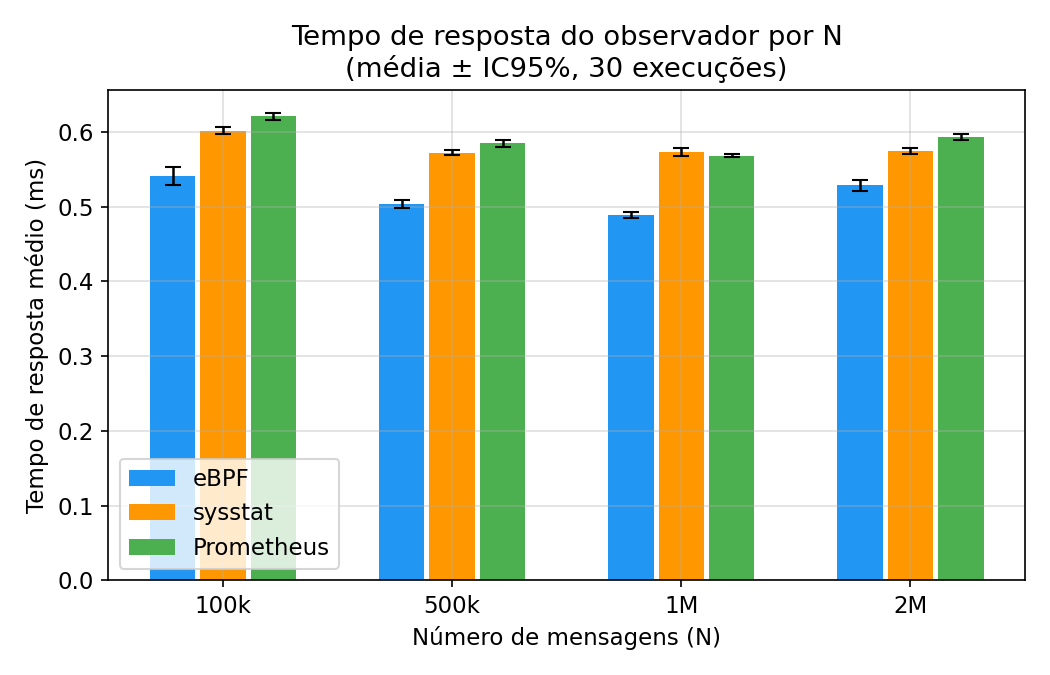
\includegraphics[width=0.85\textwidth]{imagens/tempo_resposta_por_n.png}
    \caption{Tempo de resposta médio do observador por volume de mensagens.}
    \label{fig:rtt_barras}
\end{figure}

O eBPF apresentou o menor tempo de resposta em todos os volumes avaliados. As reduções em relação ao Sysstat variaram de 8,1\% ($N = 2$ milhões) a 14,7\% ($N = 1$ milhão), e em relação ao Prometheus de 10,9\% ($N = 2$ milhões) a 14,0\% ($N = 1$ milhão). Em nenhum dos quatro volumes os intervalos de confiança de 95\% do eBPF se sobrepõem aos das demais ferramentas, indicando que a vantagem observada é estatisticamente significativa ao nível $\alpha = 0{,}05$. Esse comportamento é coerente com a natureza da abordagem: o coletor eBPF lê contadores previamente acumulados em mapas no \textit{kernel}, sem efetuar varreduras de arquivos do \texttt{/proc} nem serializar as métricas a cada requisição, ao passo que os coletores Sysstat e Prometheus realizam, a cada requisição, a leitura e o \textit{parsing} de \texttt{/proc/net/dev} e a consulta a \texttt{psutil} no espaço de usuário.

Entre Sysstat e Prometheus, as diferenças são pequenas e nem sempre consistentes: o Prometheus foi ligeiramente mais lento em três dos quatro volumes, o que é compatível com o custo adicional de manter o servidor HTTP ativo. Em $N = 1$ milhão, contudo, os dois coletores praticamente se igualaram ($0{,}5725$ \textit{vs.} $0{,}5682$ ms), com intervalos de confiança sobrepostos, de modo que não se pode afirmar diferença significativa entre eles nesse ponto.

Observa-se também que o tempo de resposta não cresce de forma monotônica com o volume de mensagens. Para as três ferramentas, os menores valores ocorrem em volumes intermediários ($N = 500$ mil e $N = 1$ milhão), enquanto $N = 100$ mil apresenta os maiores tempos médios. Esse efeito decorre da curta duração das execuções de menor volume, em que a fase de inicialização e estabilização do \textit{cache} representa fração maior do experimento; com volumes maiores, o sistema opera por mais tempo em regime estacionário, reduzindo a média.

A Figura~\ref{fig:rtt_boxplot} detalha a distribuição das execuções por meio de diagramas de caixa. Confirma-se a separação clara entre o eBPF e os demais coletores: em $N = 500$ mil e $N = 1$ milhão, a caixa do eBPF situa-se inteiramente abaixo das caixas de Sysstat e Prometheus, sem sobreposição. Nota-se, por outro lado, que o eBPF apresenta maior dispersão entre execuções, caixas mais largas e \textit{outliers} ocasionais, como o valor máximo de $1{,}0622$ ms em $N = 2$ milhões, enquanto os coletores em espaço de usuário exibem distribuições mais concentradas. Ainda assim, mesmo seus piores casos típicos permanecem competitivos com a mediana das demais ferramentas.

\begin{figure}[htbp]
    \centering
    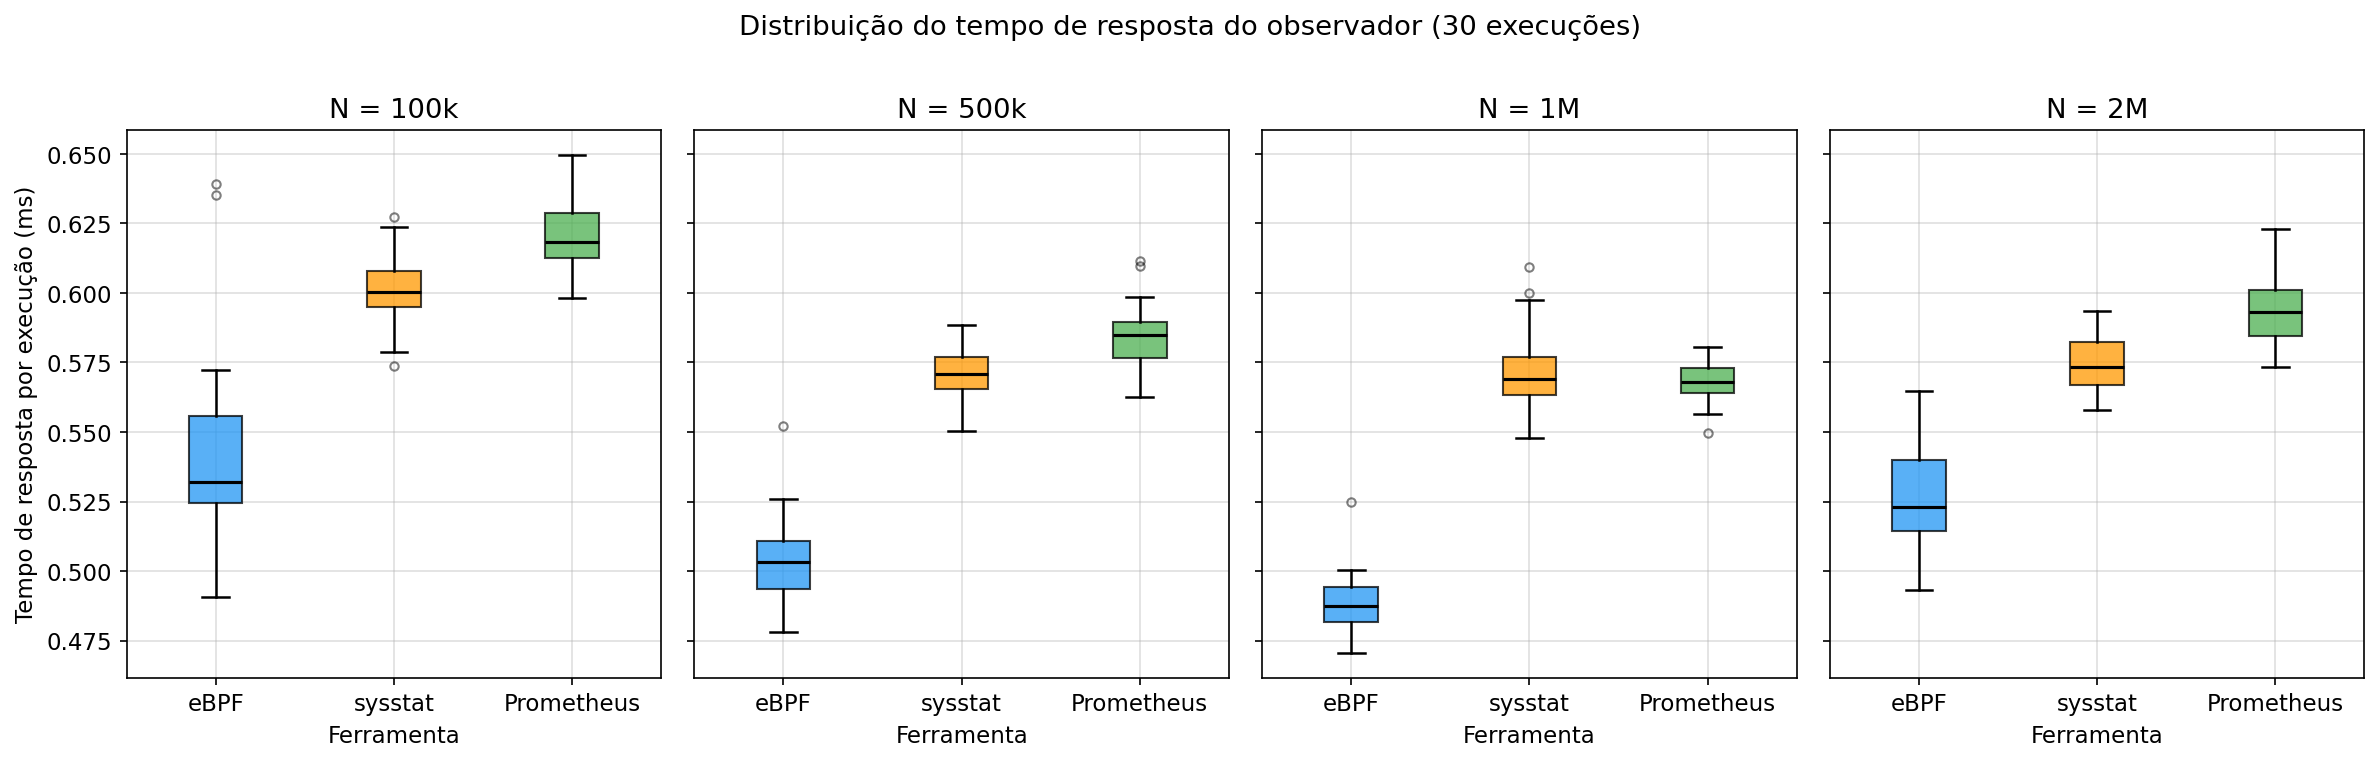
\includegraphics[width=\textwidth]{imagens/boxplot_tempo_resposta.png}
    \caption{Distribuição do tempo de resposta do observador por ferramenta e volume de mensagens.}
    \label{fig:rtt_boxplot}
\end{figure}

\FloatBarrier
\section{Consumo de CPU do WAF}

O consumo de CPU do processo WAF reflete o custo da inspeção de tráfego, idêntico nos três cenários por se tratar da mesma implementação. A Figura~\ref{fig:cpu_waf} mostra que, a partir de $N = 500$ mil, o WAF satura em torno de 107--109\% de uma \textit{thread} (valores superiores a 100\% indicam uso de mais de um núcleo lógico pelo \texttt{ThreadPoolExecutor}), sem diferença prática entre os coletores: os intervalos de confiança se sobrepõem em todos os volumes a partir desse ponto.

\begin{figure}[htbp]
    \centering
    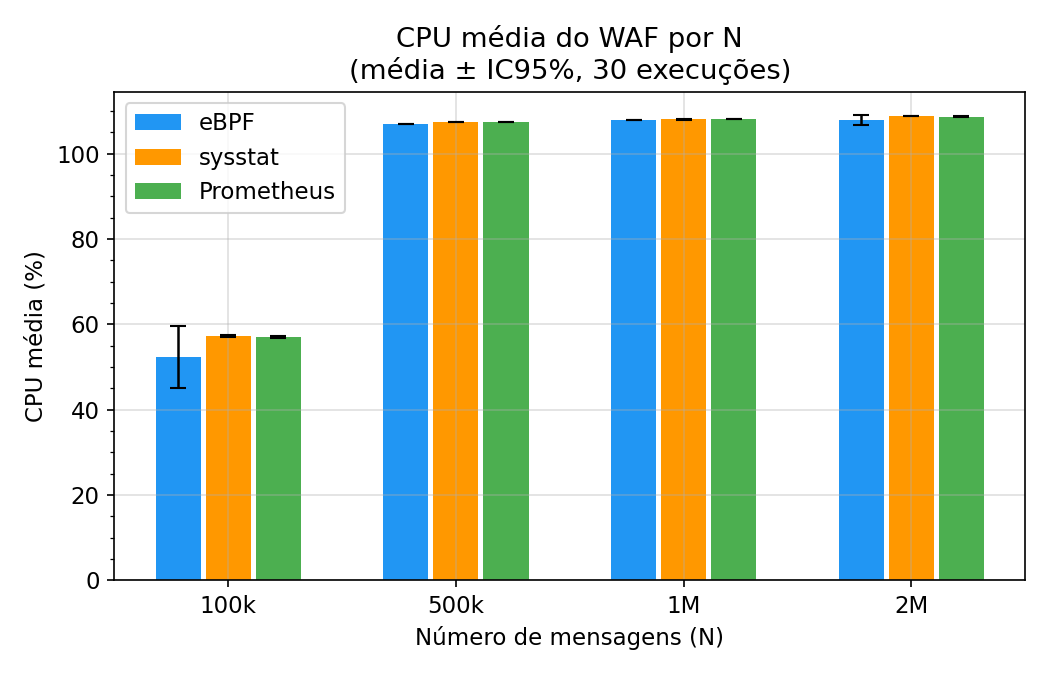
\includegraphics[width=0.85\textwidth]{imagens/cpu_waf.png}
    \caption{Consumo médio de CPU do processo WAF por volume de mensagens.}
    \label{fig:cpu_waf}
\end{figure}

A única exceção ocorre em $N = 100$ mil, em que o eBPF registrou um consumo médio de CPU inferior ($52{,}39\%$ contra $57{,}23\%$ do Sysstat e $57{,}04\%$ do Prometheus). Contudo, esse valor vem acompanhado de elevado intervalo de confiança ($\pm 7{,}28$, ante $\pm 0{,}20$ e $\pm 0{,}16$ das demais), refletindo a grande variabilidade do consumo de CPU em execuções curtas, em que o WAF não chega a operar em regime de saturação. Dada a sobreposição com a faixa de variação das outras ferramentas, não é possível atribuir essa diferença ao coletor. Em síntese, o consumo de CPU do WAF é dominado pela carga de inspeção e independe da abordagem de monitoramento adotada, resultado esperado, uma vez que nenhum dos coletores interfere no caminho de processamento das requisições.

\section{Consumo de Memória}

Esta seção analisa duas memórias distintas, com finalidades diferentes. A memória de interesse comparativo é a do \emph{próprio observador}: ela constitui o \textit{footprint} permanente da ferramenta de monitoramento --- a sobrecarga de memória que o coletor impõe apenas por estar em execução --- e é a dimensão em que as três abordagens mais se distinguem, o que justifica seu papel de variável dependente central (cf. Seção~\ref{subsec:requisitos_monitoramento}). A memória do WAF, por sua vez, é reportada como controle: por ser inerente à VNF e decorrer da mesma implementação em todos os cenários, serve para confirmar que a escolha do coletor não altera o consumo da função monitorada.

A Figura~\ref{fig:mem_observador} apresenta o consumo médio de memória RSS do processo observador, métrica em que se observa a separação mais nítida entre as três abordagens. O coletor Prometheus consome de $24{,}2$ a $24{,}8$ MB, aproximadamente 78\% acima do Sysstat ($13{,}5$ a $13{,}9$ MB) e 60\% acima do eBPF ($15{,}1$ a $15{,}2$ MB). Esse acréscimo decorre diretamente da biblioteca \texttt{prometheus\_client} e do servidor HTTP mantido em execução na porta 8000, ausentes nas demais abordagens.

\begin{figure}[htbp]
    \centering
    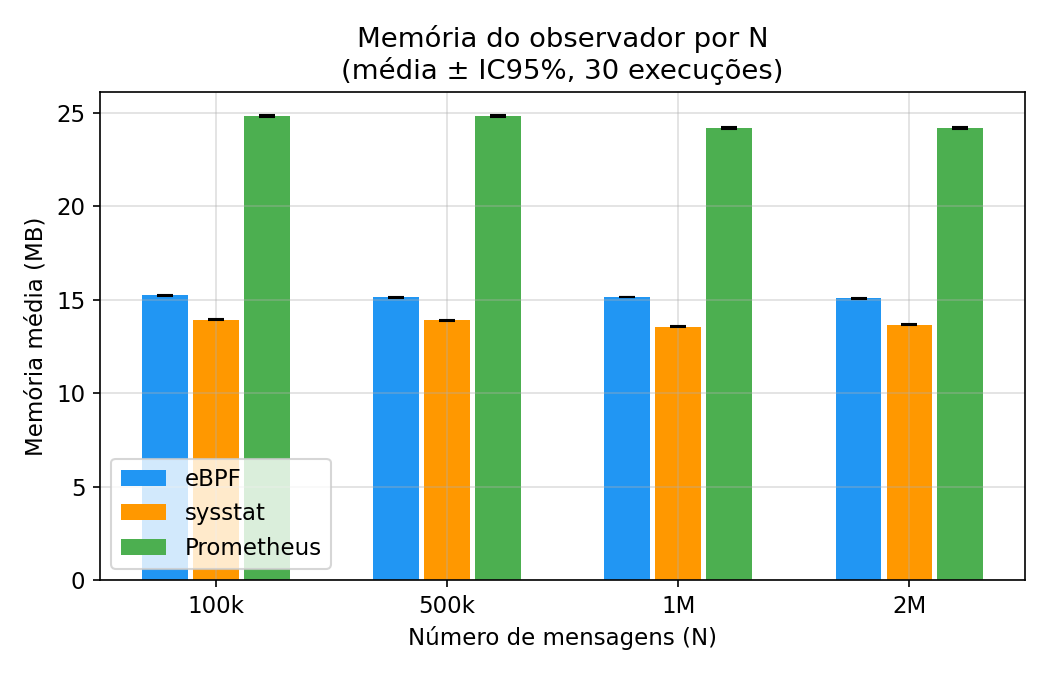
\includegraphics[width=0.85\textwidth]{imagens/memoria_observador.png}
    \caption{Consumo médio de memória RSS do processo observador por volume de mensagens (média $\pm$ IC95\%, 30 execuções).}
    \label{fig:mem_observador}
\end{figure}

Destaca-se que o consumo de memória de todos os coletores é praticamente constante ao longo dos quatro volumes de mensagens, com intervalos de confiança estreitos (inferiores a $0{,}2$ MB). Isso confirma que a memória do observador é determinada pela arquitetura de cada ferramenta, e não pelo volume de tráfego processado, comportamento esperado, dado que os coletores mantêm apenas contadores agregados e não armazenam o histórico de mensagens. O Sysstat apresentou o menor consumo, por depender unicamente de leituras de \texttt{/proc} e da biblioteca \texttt{psutil}; o eBPF situa-se ligeiramente acima, devido ao carregamento do programa BPF e dos mapas no \textit{kernel} pela \textit{libbpf}.

Quanto à memória do próprio WAF --- a VNF monitorada ---, os três cenários apresentaram valores semelhantes, crescendo de cerca de $28$ MB ($N = 100$ mil) para aproximadamente $50$ MB ($N = 2$ milhões), sem diferença atribuível ao coletor empregado. Esse crescimento acompanha o volume de tráfego processado e é inerente à VNF, não ao monitoramento, confirmando o papel de controle dessa medição.

\section{Consumo de CPU do Observador}

O consumo de CPU do próprio observador mostrou-se a métrica de medição mais delicada, devido à sua baixa magnitude frente ao ruído de amostragem. O resultado mais limpo foi obtido em $N = 100$ mil: o coletor eBPF consumiu, em média, apenas $0{,}05\% \pm 0{,}01$ de CPU, valor uma a duas ordens de grandeza inferior ao dos coletores em espaço de usuário ($4{,}66\%$ no Sysstat e $2{,}37\%$ no Prometheus) e, sobretudo, muito mais estável. Esse contraste é compatível com o argumento central de que a leitura de contadores diretamente dos mapas do \textit{kernel} é mais barata, em termos de CPU, do que a leitura periódica e o \textit{parsing} de arquivos do \texttt{/proc}; contudo, os intervalos de confiança do Sysstat ($\pm 6{,}54$) e do Prometheus ($\pm 4{,}72$) incluem o valor do eBPF, de modo que a diferença não é estatisticamente significativa.

Nos volumes maiores, entretanto, as medições de CPU do observador apresentaram desvios-padrão muito elevados em relação às médias (por exemplo, $0{,}82\% \pm 1{,}58$ no eBPF em $N = 1$ milhão), o que as torna pouco conclusivas isoladamente. Essa instabilidade decorre da granularidade da amostragem via \texttt{psutil} sobre intervalos curtos e da contenção de CPU entre os contêineres que compartilham os mesmos núcleos, conforme apontado nas limitações da metodologia. Por esse motivo, o consumo de CPU do observador é interpretado neste trabalho como evidência qualitativa complementar, e não como base para comparações quantitativas precisas entre as ferramentas.

\section{Métricas de Validação}

Além das métricas de comparação, registraram-se as métricas de validação descritas na metodologia, cujo objetivo é confirmar que as três ferramentas observaram a mesma carga de trabalho, e não discriminar as abordagens. O tempo médio de inspeção por carga convergiu para aproximadamente $0{,}081$ ms nas três abordagens (em $N = 1$ milhão, $0{,}0808$ ms no eBPF, $0{,}0815$ ms no Sysstat e $0{,}0807$ ms no Prometheus), confirmando que o custo unitário de processamento do WAF independe do coletor empregado --- comportamento esperado, dado que nenhuma abordagem interfere no caminho de inspeção das requisições.

Os contadores de bytes RX/TX, por outro lado, não são diretamente comparáveis entre as ferramentas, em razão da diferença no ponto de coleta. O coletor eBPF contabiliza exclusivamente o tráfego do WAF (porta de origem 8080), resultando em valores fortemente assimétricos --- em $N = 1$ milhão, cerca de $592$ MB recebidos contra apenas $8$ MB transmitidos, coerente com requisições volumosas e respostas curtas (\texttt{ALLOWED:OK} ou \texttt{BLOCKED}). Já o Sysstat e o Prometheus medem todo o tráfego da interface de \textit{loopback}, em que cada byte transmitido é também contabilizado como recebido, produzindo valores simétricos e mais elevados (RX $=$ TX, aproximadamente $618$ e $635$ MB, respectivamente). Essa diferença é inerente ao escopo de medição de cada abordagem, e não a um erro de contabilização; por isso, os bytes RX/TX são empregados apenas para caracterização, e não como critério de comparação entre as ferramentas.

\section{Síntese dos Resultados}

A Tabela~\ref{tab:sintese} resume o desempenho das três abordagens nas dimensões avaliadas. O eBPF foi a ferramenta de menor sobrecarga na métrica primária (tempo de resposta) em todos os volumes, com diferença estatisticamente significativa. Na CPU do próprio observador, as diferenças entre as ferramentas não foram conclusivas, devido à alta variabilidade entre as execuções. O Sysstat destacou-se pelo menor consumo de memória, enquanto o Prometheus apresentou o maior custo de memória, em razão do servidor HTTP, sem oferecer vantagem de desempenho no escopo testado, no qual o \textit{endpoint} de métricas permanece disponível, mas não é raspado ativamente.

\begin{table}[htbp]
\centering
\caption{Síntese comparativa das três abordagens de monitoramento.}
\label{tab:sintese}
\begin{tabularx}{\textwidth}{lXXX}
\hline
\textbf{Dimensão} & \textbf{eBPF} & \textbf{Sysstat} & \textbf{Prometheus} \\
\hline
Tempo de resposta (RTT UDP) & Menor & Intermediário & Maior \\
CPU do WAF & Equivalente & Equivalente & Equivalente \\
Memória do observador & Intermediária ($\sim$15 MB) & Menor ($\sim$14 MB) & Maior ($\sim$24 MB) \\
CPU do observador & Inconclusiva (mais estável em $N = 100$ mil) & Inconclusiva (ruidosa) & Inconclusiva (ruidosa) \\
\hline
\end{tabularx}
\end{table}

Os resultados confirmam a hipótese formulada na introdução: por operar em nível de \textit{kernel}, o eBPF apresenta menor tempo de resposta na coleta de métricas em comparação às abordagens de \textit{polling} em espaço de usuário, sem impor sobrecarga adicional ao WAF monitorado. A vantagem do eBPF no tempo de resposta, embora consistente e estatisticamente significativa, é de magnitude moderada (8\% a 15\%) e acompanhada de maior variabilidade entre execuções, fatores que devem ser ponderados na escolha da ferramenta em conjunto com os requisitos operacionais de cada cenário, discutidos no capítulo seguinte.
